\documentclass{article}
\usepackage{amsmath}
\usepackage{amsthm}
\usepackage{amsfonts}
\usepackage{bm}
\usepackage[usenames,dvipsnames]{xcolor}
\usepackage{tikz}
\usepackage{hyperref}

\hypersetup{
    colorlinks,
    linkcolor={red!30!black},
    citecolor={blue!50!black},
    urlcolor={blue!80!black}
}


\begin{document}


\title{Markov's inequality}
\author{ \vspace{-10ex} }
\date{ \vspace{-10ex} }
\maketitle

\section{Computing expectation from the CDF}

The cumulative distribution function (CDF) is defined as
$$
F_X(x) \equiv \operatorname{Pr}(X \le x).
$$
The complementary CDF is defined as
$$
F^c_X(x) \equiv \operatorname{Pr}(X \ge x) = 1 - F_X(x).
$$

There is an interesting theorem of computing the average
from the complementary CDF:
\begin{align}
\mathbb{E}[X] &= \int_0^\infty \operatorname{Pr}(X \ge x) \, dx.
\label{eq:avccdf}
\end{align}

\begin{proof}
Since the probability density is
$$
p_X(x) = - \frac{ d \operatorname{Pr}(X\ge x) }{ d x }.
$$
So the expected value
$$
\begin{aligned}
\mathbb{E}[X] &= \int_0^\infty x \, p_X(x) \, dx
 = -\int_0^\infty x \, d \operatorname{Pr}(X \ge x) \\
 &= -x \, \operatorname{Pr}(X\ge x) \Bigr|_0^\infty
  + \int_0^\infty \operatorname{Pr}(X \ge x) \, dx \\
 &= \int_0^\infty \operatorname{Pr}(X \ge x) \, dx.
\end{aligned}
$$
\begin{figure}[h]
  \centering
  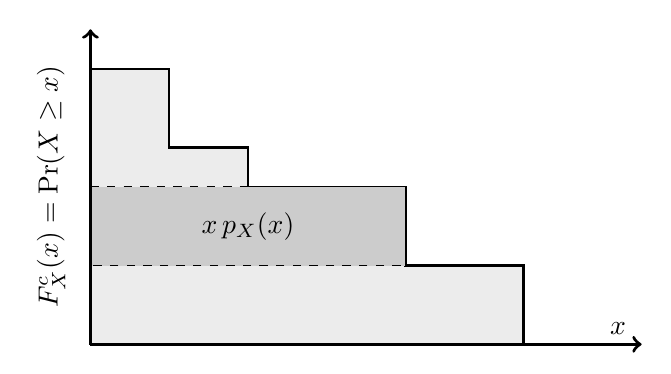
\begin{tikzpicture}
    \draw [thick, fill=gray!15!white]
      (0, 3.5) -- (1.0, 3.5) -- (1.0, 2.5)
               -- (2.0, 2.5) -- (2.0, 2.0)
               -- (4.0, 2.0) -- (4.0, 1.0)
               -- (5.5, 1.0) -- (5.5, 0.0)
               -- (0.0, 0.0) -- cycle;
    \draw [dashed, fill=black!20!white]
      (0.0, 2.0) -- (4.0, 2.0) -- (4.0, 1.0) -- (0.0, 1.0) -- cycle;

    \draw [very thick, ->] (0,0) -- (7, 0);
    \draw [very thick, ->] (0,0) -- (0, 4.0);
    \node [rotate=90] at (-0.5, 2.0) {$F_X^c(x) = \operatorname{Pr}(X \ge x)$};
    \node [] at (6.7, 0.2) {$x$};
    \node [] at (2.0, 1.5) {$x \, p_X(x)$};
  \end{tikzpicture}
\end{figure}
Geometrically, it means that the expectation can be computed from
the area under the curve of $F^c_X(x) = \operatorname{Pr}(X \ge x)$.
\end{proof}

\section{Probability inequalities}

\subsection{Markov's inequality}

For a nonnegative random variable $Y$, we have Markov's inequality
\begin{equation}
\operatorname{Pr}(Y\ge y) \le \frac{ \mathbb{E}(Y) } { y }.
\label{eq:markov_eq}
\end{equation}

\begin{proof}
From Eq. \eqref{eq:avccdf}, we get
$$
\begin{aligned}
\mathbb{E}[Y] = \int_0^\infty \operatorname{Pr}(Y \ge y) \, dy.
\end{aligned}
$$
This means that $\mathbb{E}[Y]$ is the area under the curve $\operatorname{Pr}(Y\ge y)$,
which is a function decreasing from $1$ at $y = 0$ to $0$ at $y = \infty$.
%
Now $\operatorname{Pr}(Y\ge y)$ is the area of the rectangle from $(0, 0)$
to $(y, \operatorname{Pr}(Y\ge y))$.
%
\begin{figure}[h]
  \centering
  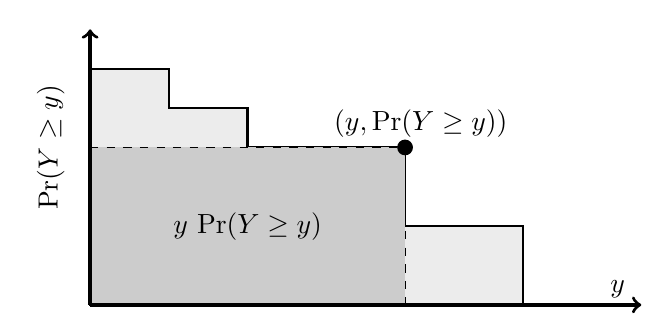
\begin{tikzpicture}
    \draw [thick, fill=gray!15!white]
      (0, 3.0) -- (1.0, 3.0) -- (1.0, 2.5)
               -- (2.0, 2.5) -- (2.0, 2.0)
               -- (4.0, 2.0) -- (4.0, 1.0)
               -- (5.5, 1.0) -- (5.5, 0.0)
               -- (0.0, 0.0) -- cycle;
    \draw [dashed, fill=black!20!white]
      (0.0, 2.0) -- (4.0, 2.0) -- (4.0, 0.0) -- (0.0, 0.0) -- cycle;

    \draw [very thick, ->] (0,0) -- (7, 0);
    \draw [very thick, ->] (0,0) -- (0, 3.5);
    \node [rotate=90] at (-0.5, 2.0) {$\operatorname{Pr}(Y \ge y)$};
    \node [] at (6.7, 0.2) {$y$};
    \node [] at (2.0, 1.0) {$y \, \operatorname{Pr}(Y \ge y)$};
    \node [] at (4.2, 2.3) {$(y, \operatorname{Pr}(Y \ge y))$};
    \node [circle, minimum size=0.2cm, inner sep=0cm, fill=black] at (4.0, 2.0){};
  \end{tikzpicture}
\end{figure}
%
This area is obviously no greater than the area represented by $\mathbb{E}[Y]$.
So
%
$$
y \, \operatorname{Pr}(Y \ge y) \le \mathbb{E}[Y],
$$
as is to be shown.
\end{proof}

Now Markov's inequality applies to not only
the original random variable $X$, but also a derived one $Y = Y(X)$
that is a function of $X$.
Two interesting examples are shown below.

\subsection{Chebyshev's inequality}

If $Z$ has a mean $\mathbb{E}[Z] = \overline Z$
and a variance, $\sigma_Z^2$, then for any $\epsilon > 0$,
we have Chebyshev's inequality.
\begin{equation}
\operatorname{Pr}\Bigl\{\bigl|Z - \overline Z \bigr|\ge \epsilon\Bigr\} \le \frac{\sigma_Z^2}{\epsilon^2}.
\label{eq:chebyshev_ineq}
\end{equation}

This can be shown by using Markov's inequality with $Y = (Z - \overline Z)^2$
$$
\operatorname{Pr}(Y \ge \epsilon^2)
\le
\frac{ \mathbb{E}[Y] } { \epsilon^2 }.
$$
Now
$\operatorname{Pr}(Y \ge \epsilon^2) = \operatorname{Pr}(|Z - \overline Z| \ge \epsilon)$,
and
$\mathbb{E}[Y] = \sigma_Z^2$,
so we get Eq. \eqref{eq:chebyshev_ineq}.

This inequality shows that the deviation drops at least as fast as $1/\epsilon^2$.


\subsection{Chernoff's inequality}

Similarly for a positive random variable $Z$, and $r > 0$, the average of
the generating function $g_Z(r) = \mathbb{E}[e^{rZ}]$, if exists, satisfies
the Chernoff bound
\begin{equation}
\operatorname{Pr}(Z \ge z)
\le g_Z(r) \, \exp(-rz).
\label{eq:chernoff_ineq}
\end{equation}

Using Markov's inequality for $Y e^{rZ}$ we get
$$
\operatorname{Pr}(Y \ge e^{rz})
\le
\frac{ \mathbb{E}[Y] } { e^{rz} }.
$$
But $\operatorname{Pr}(Y \ge e^{rz}) = \operatorname{Pr}(Z \ge z)$,
and $\mathbb{E}[Y] = g_Z(r)$, so Eq. \eqref{eq:chernoff_ineq} is proven.

This shows that the distribution tail decays exponentially as $\exp(-rz)$.
This is what makes this bound useful.


\subsection{A paradox}

In a similar manner, we can ``prove'' that, for any $r, e \ge 0$,
$$
\operatorname{Pr}(Z \ge z)
\le
\mathbb{E}[rZ^e] \, \exp(-rz^e).
$$
For example, by taking $r = 1$ and $e = 4$,
the distribution tail drops off at least as fast as $\exp(-z^4)$.
%
But this is obviously wrong for the Gaussian distribution
whose tail drops off as $\sim \exp\left( -\frac{1}{2} x^2 \right)$.

What went wrong is that the expectation $\mathbb{E}[rZ^e]$
might not exist, which breaks the deal.
%
Take another example, the Lorentz distribution
$$
p_X(x) = \frac{1}{\pi} \frac{1}{x^2 + 1}
$$
does not satisfy the Chebyshev's inequality because
it has not variance!

\section{References}

[From Robert Gallager's third lecture on stochastic process,

YouTube link: \url{https://www.youtube.com/watch?v=k0UZNZwPO8Q}.

Lecture notes: \url{http://www.rle.mit.edu/rgallager/documents/6.262lateweb1.pdf}.

See also \url{http://onlinelibrary.wiley.com/doi/10.1002/9781118593103.app2/pdf}.]



\end{document}
